\chapter{Restrições do Projecto}
\minitoc
\section{Restrições impostas}
\subsection{Restrições de Solução}

\begin{figure}
	\centering	
	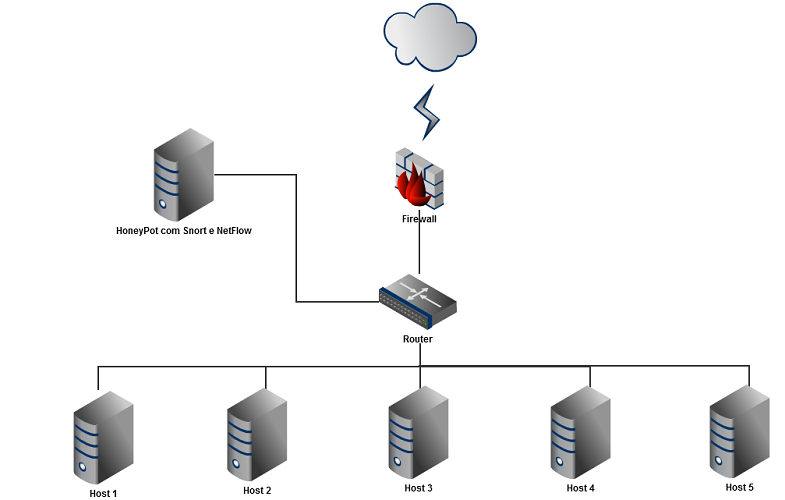
\includegraphics[scale=0.7]{images/topologia1.png}
	\caption{Topologia de Rede 1}
\end{figure}

\begin{figure}
	\centering	
	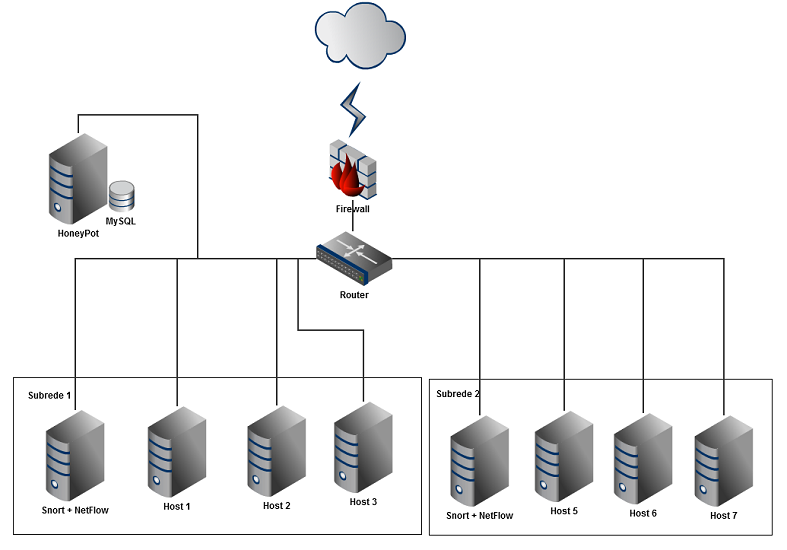
\includegraphics[scale=0.7]{images/topologia3.png}
	\caption{Topologia de Rede 2}
\end{figure}


\subsection{Ambiente de Instalação do Sistema}


Este produto é destinado a ser instalado nos servidores de cada uma das companhias de seguros compradoras. Devido a essa multiplicidade o ambiente tecnológico esperado deve manter-se universal, não contemplando nenhuma especificação particular a um determinado tipo de configuração empresarial.

\subsection{Aplicações Associadas}
Como o produto se destina a uma multiplicidade de empresas, não é possível saber com que software vai ser integrado. Contudo, para facilitar tal integração com outros \emph{softwares} da empresa, será criada uma API documentada no manual de funcionamento para promover a interacção entre este software e outros já existentes.

\subsection{Software Off-the-Shelf}
\begin{description}
    \item [Visual Paradigm for UML 7.1 Community Edition] usado para modelar o sistema de negócio e o sistema informático
    \item [Volere Template] usado como guia para elaborar o documento de requisitos

\end{description}

\subsection{Ambiente de Trabalho}
Os Utilizadores(Registado e Anónimo) do produto irão aceder ao sistema de onde pretenderem, em qualquer dispositivo electrónico que suporte o acesso \emph{web} e a tecnologia Java.

Os Mediadores executarão as suas funções laborais maioritariamente no seu local de trabalho (delegações, call-center), assim como os Colaboradores. No entanto, poderão também executá-las nos mesmos moldes que os Utilizadores anteriormente descritos.

Como este simulador de seguros não recebe nem é afectado por qualquer \emph{input} do ambiente físico exterior, estes ambientes expectáveis não terão influência directa no desenho do sistema.

\subsection{Restrições de Calendário}
\begin{description}
    \item 12 de Novembro de 2011 - Visão do Produto: 
        \begin{itemize}
            \item Análise de mercado
            \item Modelo de negócio, proposta de valor e avaliação da oportunidade
            \item Documento de Requisitos
        \end{itemize}
    \item 14 de Janeiro de 2012 - Documentação Técnica e de Instalação: 
        \begin{itemize}
            \item Produto de software
            \item Manuais de utilização
        \end{itemize}
    \item 11 de Fevereiro de 2012 : Visão Final do Produto:
        \begin{itemize}
            \item Documento de Requisitos
            \item Plano do projecto
            \item Documento do estado do projecto
            \item Documentação técnica e de instalação
            \item Produto de software
            \item Manuais de utilização
        \end{itemize}
    \item 18 de Fevereiro de 2012 : Apresentação Final: 
        \begin{itemize}
            \item Apresentação final
            \item Exposição dos trabalhos
        \end{itemize}
\end{description}

\section{Nomenclatura e Definições}
\subsection{Termos Usados no Projecto}

Ver Anexo ~\ref{appendix:1}.
